\section{实验结果}
\subsection{实验4.1-4.3}
\texttt{ws}的初值为2,0,1时的程序输出分别如图\ref{ws2},\ref{ws0},\ref{ws1}所示。

\begin{figure}[!htbp]
    \centering
    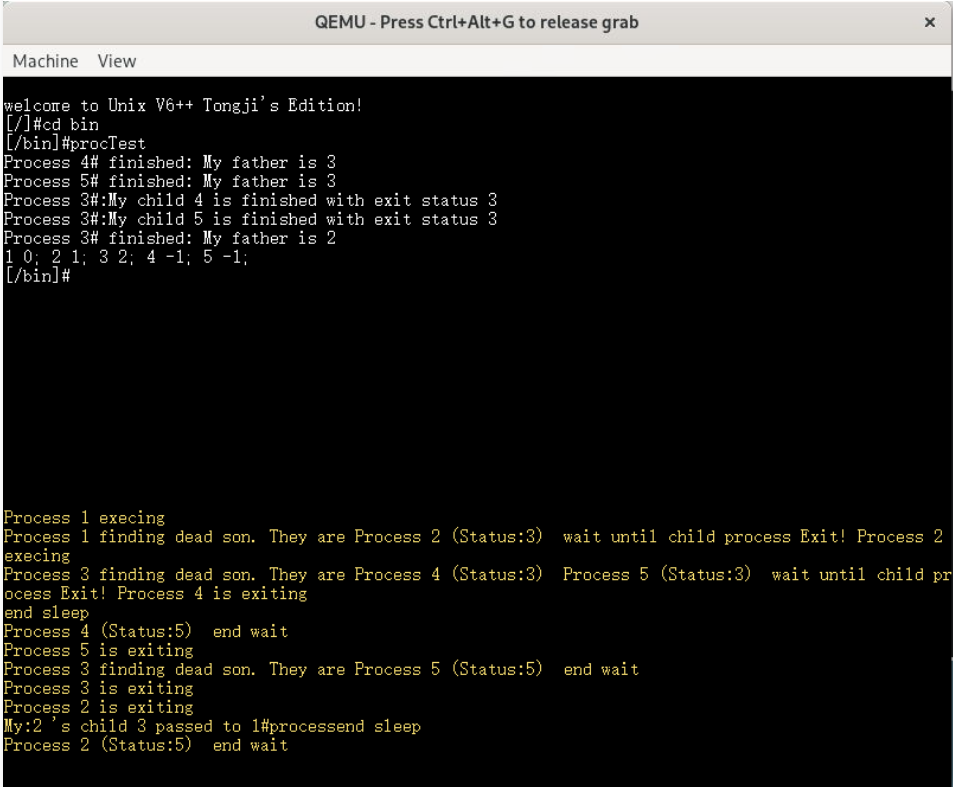
\includegraphics[width=\textwidth]{images/ws2.png}
    \caption{ws=2时的程序输出}\label{ws2}
\end{figure}

\begin{figure}[!htbp]
    \centering
    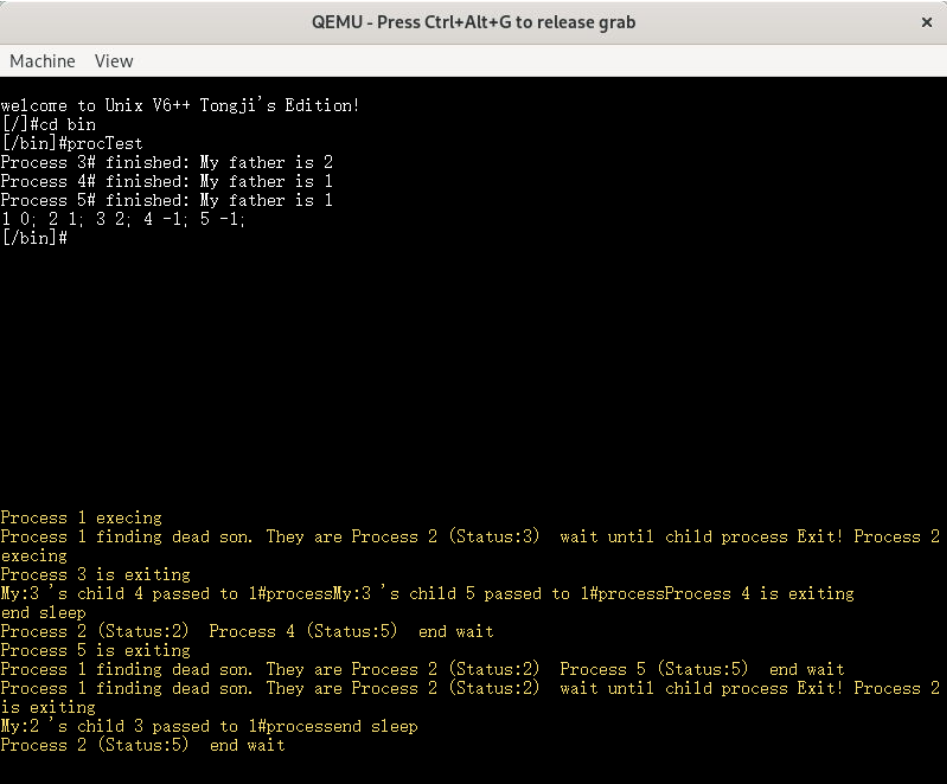
\includegraphics[width=\textwidth]{images/ws0.png}
    \caption{ws=0时的程序输出}\label{ws0}
\end{figure}

\begin{figure}[!htbp]
    \centering
    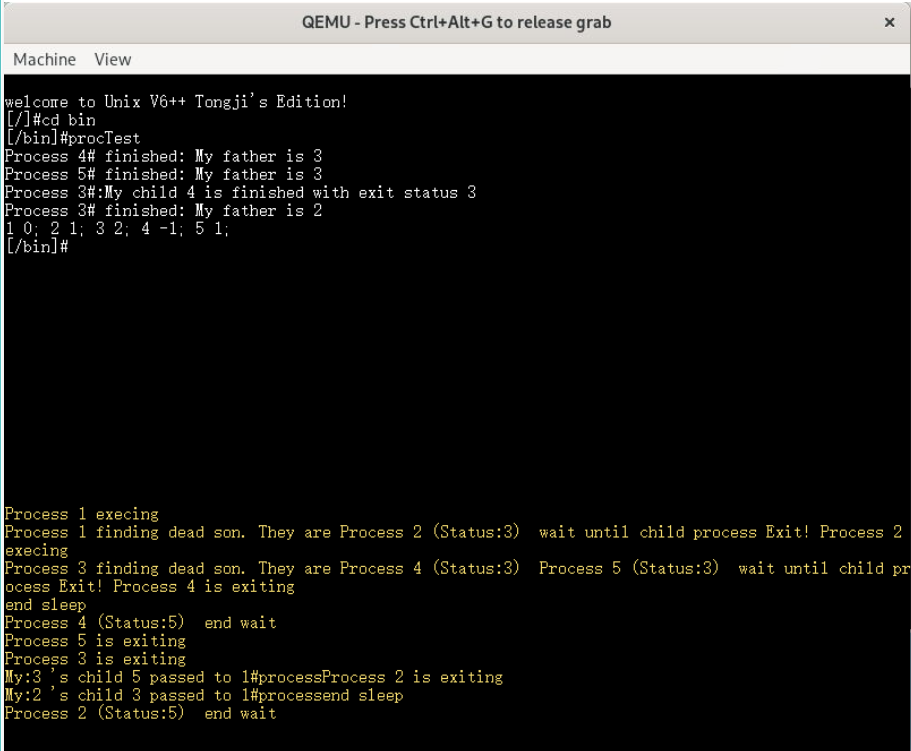
\includegraphics[width=\textwidth]{images/ws1.png}
    \caption{ws=1时的程序输出}\label{ws1}
\end{figure}

\subsection{实验4.3的解释}


实验4.3的解释如表\ref{table:ws1}所示。

\onecolumn
\begin{landscape}
    % \centering
    \begin{table}
        \centering
    \caption{ws=1时的情况分析}\label{table:ws1}
    \vspace{-10mm}
    \end{table}
     \begin{longtable}{llllll}
        \toprule
    1\#进程 &        2\#进程  & 3\#进程    & 4\#进程    & 5\#进程     & 说明\\\midrule
     \endfirsthead
        \toprule
   1\#进程  &        2\#进程  & 3\#进程    & 4\#进程    & 5\#进程     & 说明\\\midrule
     \endhead
     \bottomrule\multicolumn{6}{l}{{Continued on next page}}\\
     \endfoot
     \endlastfoot
用户态            &                     &          &           &             &            \\
\texttt{fork()}  &                      &          &           &             &  创建进程2,进程2$p\_pri\gets0$          \\
\texttt{setPri()}&                      &          &           &             &  由于运行时间短,$p\_pri$未上升,从而未设置$RunRun$   \\
用户态           &                       &          &           &             &            \\
\texttt{wait()}  &                      &          &           &             &          \\
\texttt{sleep()} &                      &          &           &             &   进程1 $p\_pri\gets40$        \\
                 &     \texttt{fork()}  &          &           &             &     \\
                 &     \texttt{setPri()}&          &           &             &  进程2$p\_pri:0\rightarrow 100,RunRun++$   \\
                 &     \texttt{Swtch()} &          &           &             &  仍选中进程2   \\
                 &     用户态            &         &           &             &            \\
                 &     \texttt{fork()}  &          &           &             & 创建进程3,进程3$p\_pri\gets0$           \\
                 &     \texttt{setPri()}&          &           &             & 由于运行时间短,进程2$p\_pri$未上升,从而未设置$RunRun$  \\
                 &     用户态            &         &           &             &            \\
                 &    \texttt{sleep(2)} &          &           &      & 进程2 $p\_pri\gets90$      \\
                 &     \texttt{Swtch()} &          &           &             &选中进程3                  \\
                 &                      & \texttt{fork()}       &           &             &  \\
                 &                      & \texttt{setPri()}    &           &             &进程3$p\_pri:0\rightarrow 100,RunRun++$ \\
                 &                      & \texttt{Swtch()}    &           &             &选中进程3 \\
                 &                      &用户态               &           &             & \\
                 &                      & \texttt{fork()}    &           &             &创建进程4,$p\_pri\gets0$                  \\
                 &                      & \texttt{setPri()}    &           &             &由于运行时间短,$p\_pri$未上升,从而未设置$RunRun$ \\
                 &                      &用户态              &           &             & \\
                 &                      & \texttt{fork()}    &           &             &创建进程5,$p\_pri\gets0$                  \\
                 &                      & \texttt{setPri()}    &           &             &由于运行时间短,$p\_pri$未上升,从而未设置$RunRun$ \\
                 &                      &用户态               &           &             & \\
                 &                      & \texttt{wait()}    &           &             & \\
                 &                      & \texttt{Sleep()}    &           &             &进程3 $p\_pri\gets40$ \\
                 &                      & \texttt{Swtch()}    &           &             &\makecell[l]{进程4,5$p\_pri$均为0,\\选中进程4(从proc[4]开始扫描)} \\
                 &                      &     & \texttt{fork()}    &                        &\\
                 &                      &     & \texttt{setPri()}    &                        &进程4$p\_pri:0\rightarrow 100,RunRun++$ \\
                 &                      &     &\texttt{Swtch()}    &              &\makecell[l]{进程4$p\_pri=100$,\\进程5$p\_pri=0$,选中进程5(从proc[5]开始扫描)} \\
                 &                      &     &                &              \texttt{fork()}    &\\
                 &                      &     &                &              \texttt{setPri()}    &进程5$p\_pri:0\rightarrow 100,RunRun++$ \\
                 &                      &     &                &              \texttt{Swtch()}     &\makecell[l]{进程2,3在睡觉,进程4,5均为100,\\选中进程4(从proc[6]开始扫描)} \\
                 &                      &     & 用户态          &             & \\
                 &                      &     & \texttt{printf()}          &             & \texttt{Process 4\# finished: My father is 3}\\
                 &                      &     & \texttt{exit()}          &             & \\
                 &                      &     & \texttt{WakeUpAll()}          &             & \\
                 &                      &     & \texttt{SetRun()}          &             & 进程3$p\_pri=40,Curpri=100,RunRun++$\\
                 &                      &     & \texttt{Swtch()}          &             &\makecell[l]{进程3$p\_pri=40$,\\进程5$p\_pri=100$,选中进程3}\\
                 &                      & \texttt{wait()}    &           &             & 释放进程4\\
                 &                      & \texttt{setPri()}    &           &             &进程3$p\_pri:40\rightarrow 100,RunRun++$ \\
                 &                      & \texttt{Swtch()}    &           &             & \makecell[l]{进程3,5$p\_pri$均为100\\选中进程5(从proc[4]开始扫描)}\\
                 &                      &     &                &             用户态    & \\
                 &                      &     &                &            \texttt{printf()}    & \texttt{Process 5\# finished: My father is 3}\\
                 &                      &     &                &            \texttt{exit()}    & \\
                 &                      &     &                &            \texttt{WakeUpAll()} &父进程3不在睡觉 \\
                 &                      &     &                &            \texttt{Swtch()}    & 选取进程3\\
                 &                      &用户态   &           &             & \\
                 &                      &\texttt{printf()}   &           &             &\texttt{Process 3\#:My child 4 is finished with exit status 3} \\
                 &                      &\texttt{printf()}   &           &             &\texttt{Process 3\#: finished: My father is 2} \\
                 &                      &\texttt{exit()}   &           &             &将子进程5的父进程更改为进程1\\
                 &                      &\texttt{WakeUpAll()}   &           &             &父进程2不因\texttt{wait()}睡觉\\
                 &                      &\texttt{Swtch()}   &           &             &\\
                 \multicolumn{6}{c}{此时进程1因\texttt{wait()}睡觉,进程2因\texttt{sleep(2)}睡觉,进程3,5为SZOMB状态,进程4已彻底删除,系统等待进程2被唤醒}\\
                 &                用户态 &        &           &             &\\
                 &                \texttt{printf()}   &                &           &             &\makecell[l]{进程4已被进程3释放,\\进程5已在进程3\texttt{exit}时改为进程1的子进程}\\
                 &                \texttt{exit()}   &                &           &             &系统自动调用,将子进程3的父进程设置为1\\
                 &                \texttt{WakeUpAll()}   &                &           &             &唤醒父进程1\\
                 &                \texttt{SetRun()}   &                &           &             &进程1$p\_pri=40,Curpri=90,RunRun++$\\
                 &                \texttt{Swtch()}   &                &           &             &选中进程1\\
                \texttt{wait()} &                  &                &           &             &释放进程2,返回值为2,符合循环退出条件\\
    \texttt{setPri()} &                  &                &           &             &进程1$p\_pri:40\rightarrow 100,RunRun++$\\
    \texttt{Swtch()} &                  &                &           &             &选中进程1\\
    用户态 &                  &                &           &             &退出循环\\\bottomrule
    \end{longtable}
\end{landscape}

\subsection{实验4.4的解释}

修改代码后分别使得父进程创建5\#前后被抢占对应的运行结果如图\ref{fig6},\ref{fig7}所示。
相应解释分别如表\ref{table:fig6},\ref{table:fig7}所示。

\begin{figure}[!htbp]
    \centering
    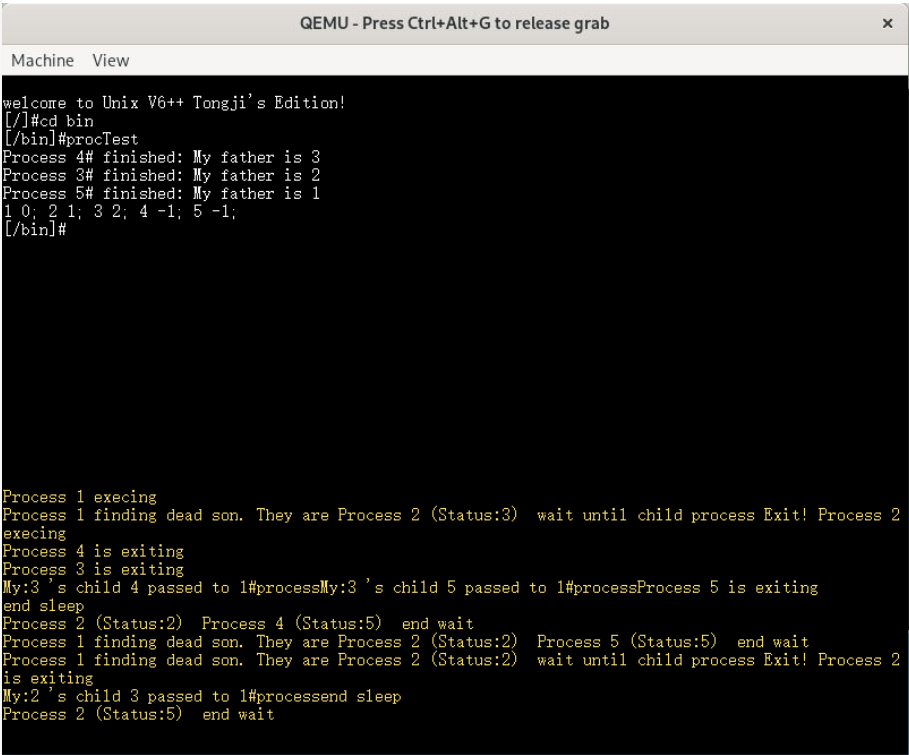
\includegraphics[width=\textwidth]{images/fig6.png}
    \caption{父进程创建5\#之前被抢占}\label{fig6}
\end{figure}

\begin{figure}[!htbp]
    \centering
    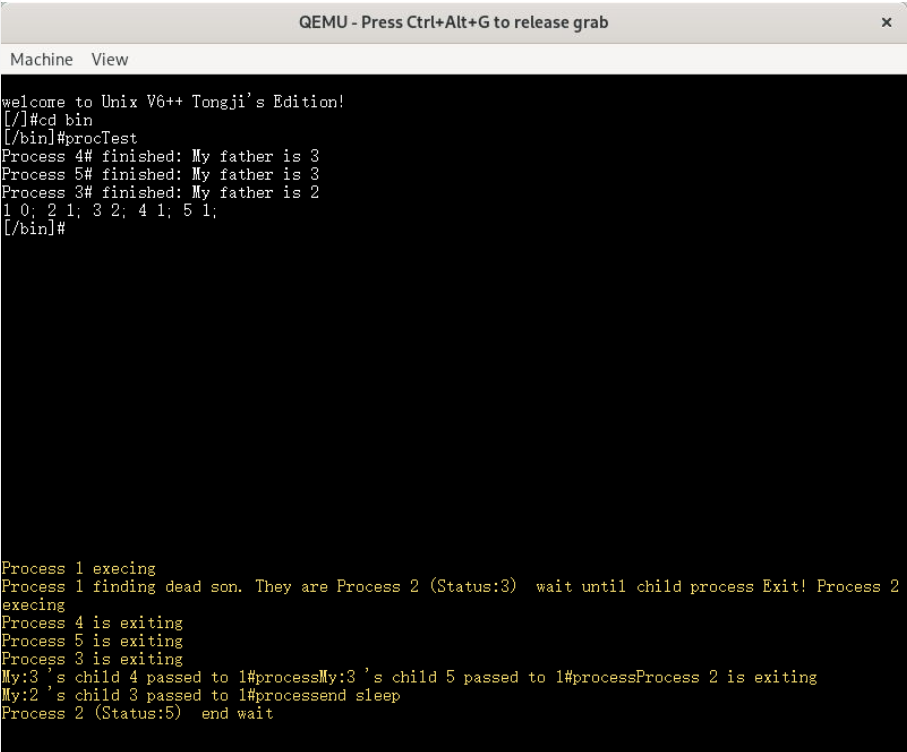
\includegraphics[width=\textwidth]{images/fig7.png}
    \caption{父进程创建5\#之后被抢占}\label{fig7}
\end{figure}

\onecolumn
\begin{landscape}
    % \centering
    \begin{table}
        \centering
    \caption{父进程创建5\#之前被抢占}\label{table:fig6}
    \vspace{-10mm}
    \end{table}
     \begin{longtable}{llllll}
        \toprule
    1\#进程 &        2\#进程  & 3\#进程    & 4\#进程    & 5\#进程     & 说明\\\midrule
     \endfirsthead
        \toprule
   1\#进程  &        2\#进程  & 3\#进程    & 4\#进程    & 5\#进程     & 说明\\\midrule
     \endhead
     \bottomrule\multicolumn{6}{l}{{Continued on next page}}\\
     \endfoot
     \endlastfoot
用户态            &                     &          &           &             &            \\
\texttt{fork()}  &                      &          &           &             &  创建进程2,进程2$p\_pri\gets0$          \\
\texttt{setPri()}&                      &          &           &             &  由于运行时间短,$p\_pri$未上升,从而未设置$RunRun$   \\
用户态           &                       &          &           &             &            \\
\texttt{wait()}  &                      &          &           &             &          \\
\texttt{sleep()} &                      &          &           &             &   进程1 $p\_pri\gets40$        \\
                 &     \texttt{fork()}  &          &           &             &     \\
                 &     \texttt{setPri()}&          &           &             &  进程2$p\_pri:0\rightarrow 100,RunRun++$   \\
                 &     \texttt{Swtch()} &          &           &             &  仍选中进程2   \\
                 &     用户态            &         &           &             &            \\
                 &     \texttt{fork()}  &          &           &             & 创建进程3,进程3$p\_pri\gets0$           \\
                 &     \texttt{setPri()}&          &           &             & 由于运行时间短,进程2$p\_pri$未上升,从而未设置$RunRun$  \\
                 &     用户态            &         &           &             &            \\
                 &    \texttt{sleep(2)} &          &           &      & 进程2 $p\_pri\gets90$      \\
                 &     \texttt{Swtch()} &          &           &             &选中进程3                  \\
                 &                      & \texttt{fork()}       &           &             &  \\
                 &                      & \texttt{setPri()}    &           &             &进程3$p\_pri:0\rightarrow 100,RunRun++$ \\
                 &                      & \texttt{Swtch()}    &           &             &选中进程3 \\
                 &                      &用户态               &           &             & 执行计算任务\\
                 &                      & \texttt{fork()}    &           &             &创建进程4,$p\_pri\gets0$                  \\
                 &                      & \texttt{setPri()}    &           &             &由于执行计算任务,$p\_pri$上升,从而设置$RunRun$ \\

                 &                      & \texttt{Swtch()}    &           &             & \makecell[l]{进程3$p\_pri$大于进程4$p\_pri$\\进程4上台}\\
                 &                      &     & \texttt{fork()}    &                        &\\
                 &                      &     & \texttt{setPri()}    &                        &进程4$p\_pri:0\rightarrow 100,RunRun++$ \\
                 &                      &     &\texttt{Swtch()}    &              &\makecell[l]{进程3$p\_pri$大于进程4$p\_pri$\\进程4上台}\\
                  &                      &     & \texttt{printf()}          &             & \texttt{Process 4\# finished: My father is 3}\\
                 &                      &     & \texttt{exit()}          &             & \\
                 &                      &     & \texttt{WakeUpAll()}          &             & 父进程3不在睡觉\\
                 &                      &     & \texttt{Swtch()}          &             &选中进程3\\
                 &                      &用户态              &           &             & \\
                 &                      & \texttt{fork()}    &           &             &创建进程5,$p\_pri\gets0$                  \\
                 &                      & \texttt{setPri()}    &           &             &\makecell[l]{由于上台后未执行计算任务,\\$p\_pri$未上升,从而未设置$RunRun$} \\
                 &                      &用户态               &           &             & \\
                 &                      &\texttt{printf()}   &           &             &\texttt{Process 3\#: finished: My father is 2} \\
                 &                      &\texttt{exit()}   &           &             &将子进程4,5的父进程更改为进程1\\
                 &                      &\texttt{WakeUpAll()}   &           &             &父进程2不因\texttt{wait()}睡觉\\
                 &                      &\texttt{Swtch()}   &           &             &\\
                &                      &     &                &              \texttt{fork()}    &\\
                 &                      &     &                &              \texttt{setPri()}    &进程5$p\_pri:0\rightarrow 100,RunRun++$ \\
                 &                      &     &                &              \texttt{Swtch()}     &选中进程5 \\
                 &                      &     &                &             用户态    & \\
                 &                      &     &                &            \texttt{printf()}    & \texttt{Process 5\# finished: My father is 1}\\
                 &                      &     &                &            \texttt{exit()}    & \\
                 &                      &     &                &            \texttt{WakeUpAll()} &唤醒父进程1 \\
                 &                      &     &                &            \texttt{SetRun()} & 进程1$p\_pri=40,Curpri=100,RunRun++$\\
                 &                      &     &                &            \texttt{Swtch()}    & 选取进程1\\
用户态           &                       &          &           &             &            \\
   \texttt{wait()} &                  &                &           &             &\makecell[l]{线性扫描至进程4,释放其PCB,\\返回值为4,不符合循环退出条件}\\
    \texttt{setPri()} &                  &                &           &             &进程1$p\_pri:40\rightarrow 100,RunRun++$\\
    \texttt{Swtch()} &                  &                &           &             &选中进程1\\
用户态           &                       &          &           &             &            \\
    \texttt{wait()} &                  &                &           &             &\makecell[l]{线性扫描至进程5,释放其PCB,\\返回值为4,不符合循环退出条件}\\
    \texttt{setPri()} &                  &                &           &             &进程1$p\_pri:40\rightarrow 100,RunRun++$\\
    \texttt{Swtch()} &                  &                &           &             &选中进程1\\
用户态           &                       &          &           &             &            \\
    \texttt{wait()} &                  &                &           &             &\\
\texttt{sleep()} &                      &          &           &             &      \\
                \multicolumn{6}{c}{此时进程1因\texttt{wait()}睡觉,进程2因\texttt{sleep(5)}睡觉,进程3为SZOMB状态,进程4,5已释放,系统等待进程2被唤醒}\\
                 &                用户态 &        &           &             &\\
                 &                \texttt{printf()}   &                &           &             &\\
                 &                \texttt{exit()}   &                &           &             &系统自动调用,将子进程3的父进程设置为1\\
                 &                \texttt{WakeUpAll()}   &                &           &             &唤醒父进程1\\
                 &                \texttt{SetRun()}   &                &           &             &进程1$p\_pri=40,Curpri=90,RunRun++$\\
                 &                \texttt{Swtch()}   &                &           &             &选中进程1\\
    \texttt{wait()} &                  &                &           &             &释放进程2,返回值为2,符合循环退出条件\\
    \texttt{setPri()} &                  &                &           &             &进程1$p\_pri:40\rightarrow 100,RunRun++$\\
    \texttt{Swtch()} &                  &                &           &             &选中进程1\\
    用户态 &                  &                &           &             &退出循环\\\bottomrule
    \end{longtable}
\end{landscape}

\onecolumn
\begin{landscape}
    % \centering
    \begin{table}
        \centering
    \caption{父进程创建5\#之后被抢占}\label{table:fig7}
    \vspace{-10mm}
    \end{table}
     \begin{longtable}{llllll}
        \toprule
    1\#进程 &        2\#进程  & 3\#进程    & 4\#进程    & 5\#进程     & 说明\\\midrule
     \endfirsthead
        \toprule
   1\#进程  &        2\#进程  & 3\#进程    & 4\#进程    & 5\#进程     & 说明\\\midrule
     \endhead
     \bottomrule\multicolumn{6}{l}{{Continued on next page}}\\
     \endfoot
     \endlastfoot
用户态            &                     &          &           &             &            \\
\texttt{fork()}  &                      &          &           &             &  创建进程2,进程2$p\_pri\gets0$          \\
\texttt{setPri()}&                      &          &           &             &  由于运行时间短,$p\_pri$未上升,从而未设置$RunRun$   \\
用户态           &                       &          &           &             &            \\
\texttt{wait()}  &                      &          &           &             &          \\
\texttt{sleep()} &                      &          &           &             &   进程1 $p\_pri\gets40$        \\
                 &     \texttt{fork()}  &          &           &             &     \\
                 &     \texttt{setPri()}&          &           &             &  进程2$p\_pri:0\rightarrow 100,RunRun++$   \\
                 &     \texttt{Swtch()} &          &           &             &  仍选中进程2   \\
                 &     用户态            &         &           &             &            \\
                 &     \texttt{fork()}  &          &           &             & 创建进程3,进程3$p\_pri\gets0$           \\
                 &     \texttt{setPri()}&          &           &             & 由于运行时间短,进程2$p\_pri$未上升,从而未设置$RunRun$  \\
                 &     用户态            &         &           &             &            \\
                 &    \texttt{sleep(2)} &          &           &      & 进程2 $p\_pri\gets90$      \\
                 &     \texttt{Swtch()} &          &           &             &选中进程3                  \\
                 &                      & \texttt{fork()}       &           &             &  \\
                 &                      & \texttt{setPri()}    &           &             &进程3$p\_pri:0\rightarrow 100,RunRun++$ \\
                 &                      & \texttt{Swtch()}    &           &             &选中进程3 \\
                 &                      &用户态               &           &             & \\
                 &                      & \texttt{fork()}    &           &             &创建进程4,$p\_pri\gets0$                  \\
                 &                      & \texttt{setPri()}    &           &             &由于运行时间短,$p\_pri$未上升,从而未设置$RunRun$ \\
                 &                      &用户态              &           &             & 执行计算任务\\
                 &                      & \texttt{fork()}    &           &             &创建进程5,$p\_pri\gets0$                  \\
                 &                      & \texttt{setPri()}    &           &             &由于执行计算任务,$p\_pri$上升,从而设置$RunRun$ \\
                 &                      &     & \texttt{fork()}    &                        &\\
                 &                      &     & \texttt{setPri()}    &                        &进程4$p\_pri:0\rightarrow 100,RunRun++$ \\
                 &                      &     &\texttt{Swtch()}    &              &\makecell[l]{进程4$p\_pri=100$,\\进程5$p\_pri=0$,选中进程5(从proc[5]开始扫描)} \\
                 &                      &     &                &              \texttt{fork()}    &\\
                 &                      &     &                &              \texttt{setPri()}    &进程5$p\_pri:0\rightarrow 100,RunRun++$ \\
                 &                      &     &                &              \texttt{Swtch()}     &\makecell[l]{进程3$p\_pri>100$,进程4,5均为100,\\选中进程4(从proc[6]开始扫描)} \\
                 &                      &     & 用户态          &             & \\
                 &                      &     & \texttt{printf()}          &             & \texttt{Process 4\# finished: My father is 3}\\
                 &                      &     & \texttt{exit()}          &             & \\
                 &                      &     & \texttt{WakeUpAll()}          &             &父进程3不在睡觉 \\
                 &                      &     & \texttt{Swtch()}          &             &\makecell[l]{进程3$p\_pri>$进程5$p\_pri$,选中进程5}\\
                 &                      &     &                &             用户态    & \\
                 &                      &     &                &            \texttt{printf()}    & \texttt{Process 5\# finished: My father is 3}\\
                 &                      &     &                &            \texttt{exit()}    & \\
                 &                      &     &                &            \texttt{WakeUpAll()} &父进程3不在睡觉 \\
                 &                      &     &                &            \texttt{Swtch()}    & 选取进程3\\
                 &                      &用户态               &           &             & \\
                 &                      &\texttt{printf()}   &           &             &\texttt{Process 3\#: finished: My father is 2} \\
                 &                      &\texttt{exit()}   &           &             &将子进程4,5的父进程更改为进程1\\
                 &                      &\texttt{WakeUpAll()}   &           &             &父进程2不因\texttt{wait()}睡觉\\
                 &                      &\texttt{Swtch()}   &           &             &\\
                 \multicolumn{6}{c}{此时进程1因\texttt{wait()}睡觉,进程2因\texttt{sleep(5)}睡觉,进程3,4,5为SZOMB状态,系统等待进程2被唤醒}\\
                 &                用户态 &        &           &             &\\
                 &                \texttt{printf()}   &                &           &             &\\
                 &                \texttt{exit()}   &                &           &             &系统自动调用,将子进程3的父进程设置为1\\
                 &                \texttt{WakeUpAll()}   &                &           &             &唤醒父进程1\\
                 &                \texttt{SetRun()}   &                &           &             &进程1$p\_pri=40,Curpri=90,RunRun++$\\
                 &                \texttt{Swtch()}   &                &           &             &选中进程1\\
                \texttt{wait()} &                  &                &           &             &释放进程2,返回值为2,符合循环退出条件\\
    \texttt{setPri()} &                  &                &           &             &进程1$p\_pri:40\rightarrow 100,RunRun++$\\
    \texttt{Swtch()} &                  &                &           &             &选中进程1\\
    用户态 &                  &                &           &             &退出循环\\\bottomrule
    \end{longtable}
\end{landscape}

